\documentclass[
]{ceurart}

\usepackage[utf8]{inputenc}

\begin{document}

\copyrightyear{2022}
\copyrightclause{Copyright for this paper by its authors.
  Use permitted under Creative Commons License Attribution 4.0
  International (CC BY 4.0).}

\conference{ALTNLP2022: The International Conference on Agglutinative Language Technologies as a challenge of Natural Language Processing, June 6-8, 2022, Koper, Slovenia}

\title{BoAT Web Annotation Tool for Turkish Dependency Parsing}

\author[]{Salih Furkan Akkurt}[%
email=furkan.akkurt@boun.edu.tr
]
% busra
\author[]{Suzan Uskudarli}[%
email=suzan.uskudarli@boun.edu.tr
]

\address[]{ Department of Computer Engineering, Bogazici University, Bebek, 34342, İstanbul, Turkey }

\begin{abstract}
High quality treebanks are desirable for ever-increasing number of data-driven developments.
Manual annotation of sentences in these treebanks by dependency parsing is an important but time-consuming and error-prone task.
There are various tools that try to make the task easier for annotators.
Maintaining the focus of the annotator during annotation sessions, reducing distractions and also preventing errors are important parts of these tools.
After much feedback for our initial tool BoAT for desktop, a new software requirements specification was created.
New features and improvements have been extracted from the feedback.
Autocompletion of cells, searching of annotations and APIs were selected to be the most needed improvements.
A Web application was our obvious choice for these functionalities, rather than a local GUI.
Accordingly, a search functionality serving to achieve interannotator agreement was implemented.
Searching for similar annotations is a helpful addition to the tool, making treebanks more consistent.
We also provide APIs for 3rd party usage of the annotations: searching and getting annotations.
Thus, we made a tool that tries to address and achieve these points.
% Notes from meeting
% docker, API, accessible
% reliant on language specific
% often manually produced by annotators with linguistic background; highly labour-intensive task
% annotator centric
% Turkish, morphologically-rich language [should be in abstract]
% UD should be in abstract; this tool serves multiple annotators
\end{abstract}

\begin{keywords}
natural language processing \sep
linguistic annotation \sep
annotation tool \sep
web application \sep
dependency parsing \sep
Universal Dependencies
\end{keywords}

\maketitle

\section{Introduction}
\label{sec:introduction}
Treebanks are 
Manually annotating these treebanks is an intense activity undertaken by annotators.
Several tools to support dependency parsing annotations have been developed. % citations from related work
For morphologically-rich languages like Turkish, dependency annotation tends to be much more challenging.
Turkish being an agglutinative language, words are split into further lemmas.
Parsing dependencies in such a language manually is hard work.
Tools developed with drag-drop functionalities tend to disrupt the flow state of the annotator by requiring to use a mouse in the middle of a keyboard-intensive activity.
The tool developed and used for the annotation of the BOUN Treebank had significant improvements on efficiency by making it a priority to be a keyboard-oriented application.

Annotator's experiences using the first version and other annotation tools have been taken into consideration to improve the tool further and make their experiences healthier.
Feedback have been ample for the initial standalone version regarding the user's experience.
We started to design a web-based application with a database and APIs where interannotator agreement would be smoother and automated.
By making it a web app, we increased the accessibility of the software so that it can be used for other purposes by altering it slightly.
We plan to dockerize it and make the API accessible to the 3rd parties.
The initial feedback and the tests done promise much for the future of the tool.

This paper presents this new web-based tool.
In Section~\ref{sec:related}, the related work is touched upon.
% requirements from first version
In Section~\ref{sec:requirements}, elicited and specified software requirements and design procedure is detailed.
In Section~\ref{sec:implementation}, how the implementation proceeded is explained.
Section~\ref{sec:features} explains what features the tool contains.
In Section~\ref{sec:annotation}, a use case going through an annotation of a sentence is included.
Section~\ref{sec:discussion} contemplates what the future of the tool may entail.
Section~\ref{sec:conclusion} adds the final conclusions.

\section{Related Work}
\label{sec:related}

There are many tools for annotation but many of them use a hybrid approach regarding keyboard and mice usage.
For example, brat is an open source project for text annotation on browsers.\cite{brat}\cite{UD}
There are other third-party tools presented in the UD tools webpage such as UD Annotatrix\cite{tyers-etal:2018} and DgAnnotator\cite{dgannotator}.
DgAnnotator is specifically for creating dependency trees and adding dependency relations.
UD Annotatrix is, as the name implies, a tool for UD treebanks.
It's a mouse-oriented tool, using clicks.

BoAT v1~\cite{turk-etal-2019-turkish}, is a standalone application.
It has a keyboard-oriented approach, but it lacks a network for annotators.
The annotation done on the BOUN Treebank and the feedback that came of that work indicates that keyboard-only approach is more efficient and takes less time for creating treebanks.
It was implemented for treebanks using the UD framework.
This tool has been used to annotate the entire BOUN Treebank.
We try to improve on and add new features to this tool in this paper, while making it available on the web.

\section{Requirements and Design}
\label{sec:requirements}

% Suzan, introduction sentence
In-depth interviews and requirements elicitation with annotators that have annotated the entire BOUN treebank, which has close to 10 thousand sentences, have been conducted to elicit the software requirements.
Annotators may struggle with a specific annotation and want to be able to search for specific annotations similar to the one they are currently doing to make the treebank consistent within itself and reduce their cognitive load in general.
Thus, a search functionality for annotators needs to be built with a network of annotators to allow them to cross-check each other's work.
Because there was a pressing need for a network, we decided to develop a new web-based tool from scratch.

The annotation process requires a great deal of attention, therefore, the main priority is to improve the user experience for the annotator so that they can more efficiently produce accurate annotations.
Annotators use the tools sometimes for hours on end.
Software should make the work easier by reducing distractions and automating work that can be automated.
One of the requirements we have gathered for not breaking the focus of the annotator is for the software to use only keyboard for every task.
BoAT is a keyboard-oriented application.
User should not have to use a mouse for any type of task.
Since users lose focus after some time naturally, automating the entries and checking errors are high priorities in this respect.
Autocomplete should be provided for parts of the annotation where it is known what values are allowed for a CoNLL-U type annotation.
Autocompletion reduces errors and increases efficiency.

One feature requested by annotators is using the screen space in a compact manner and removing any clutter that's not used much.
Considering this, the previous application's checkboxes have been converted into a select, leaving more space for the annotation table where most of the annotator focus is directed towards.

% good software practices; dockerize
A search API for the annotation database of the treebanks is another requirement.
An annotator should be able to search the treebank they are a part of to see other annotations done for a specific sentence or go to a sentence's annotation page to start annotating.
Sometimes a user may not be sure of an annotation and would like to consult previous annotations for similar cases.
They should be able to search the database in a complex way, by case, features or direct text, etc.
An outsider also should be able to use the API to get the annotations of a particular treebank to use in their tasks in a systematic way.

\section{Implementation}
\label{sec:implementation}

The Django\cite{django} Web application development framework and its Django REST Framework\cite{drf} were used to develop our annotation tool.
Django REST Framework were used for the API part.
% API
% backend database
% changed models for wordlines, helping API

% features
A user is able to upload a \textit{conllu} file and start annotating.
The system is responsible for checking if a file uploaded obeys the format of \textit{conllu}.
The annotation page resembles the initial standalone application.
It includes a dependency graph and an editable table, both of which in sync.
The dependency graph of the initial tool and other 2 graphs have been added to this tool.
The user has the choice to select a type of graph or none.
The other 2 graphs have been selected due to space considerations.
These graphs are horizontal and linear.
The table is responsible for changing the word lines of \textit{conllu} files.

Errors are checked and annotations validated according to the UD framework and the language provided.
The scripts used for validation are the latest ones already provided by the framework.\cite{UD-git}

PostgreSQL\cite{psql} is used to provide a database for the server-side applications of the software.
This database is responsible for serving the entire data needed to operate the tool, the search API, etc.

A Python library \textit{spaCy}\cite{spacy} is used to provide linear dependency graphs.
Another JavaScript-based linear dependency graph\cite{spyssalo} making use of brat\cite{brat-vis} is used to provide graphs as well.
The preferences of annotators may vary and giving them options in different parts of the screen is important.

% Docker

\section{Features}
\label{sec:features}

% consistent annotation
% an annotator can struggle with a specific one; search helps
% busra'dan ornek; kisa (ya da uzun gerekiyorsa)
An important feature in this version is the ability to cross-check annotations by implementing a network for annotators where they can see the annotations done by other annotators and if they disagree on some parts, they can interact outside the tool.
This can be helpful and a learning experience for annotators.

Also one other thing the interannotator agreement allows us is the possibility to see some anomalies in the Turkish part of the UD framework.
For example, if a sentence were annotated a way by many annotators but the UD validation script were giving errors for it, this might indicate the UD validation were lacking in this respect of the Turkish language.
Some modifications might be necessary and there could be a case for a proposal of change.

\subsection{API}
\label{sec:api}

By using our annotated treebank search API, other parties wanting to check out the capabilities of the tool can retrieve our annotated treebanks.
Also, some parties wanting to use the treebanks in their computation tasks can easily extract information from our treebanks by using the API.
This opens up many possibilities for the use of the tool beyond the annotator's UI experience.

\subsection{Demo}
\label{sec:demo}

A demo will be provided on our university's NLP web page where the annotation capabilities of the tool built can be tested.

\section{Annotation Procedure}
\label{sec:annotation}
This section describes how an annotator annotates a Turkish sentence.

An annotator selects a sentence from a treebank, which has previously uploaded sentences coming from a CoNLL-U formatted file.
They fill the cells of the annotation table's fields.
During the annotation, an annotator can make use of dependency graphs, error cards and the search functionality.
Dependency graphs are visual cues for how an annotation is going, using HEADs and DEPRELs.
They can choose 3 different graphs one at a time or select to hide.
Different graphs show the same information with a horizontal or vertical tree.
Errors are helpful reminders, coming from a validation script found on the UD repository.
They can use the search functionality to search for previous annotations by other annotators or themselves, using various fields (text, FEATS, etc.) for the query.
By checking similar annotations, an annotator can ensure consistency and don't lose focus by trying manual methods for the same information.
When an annotation is done, they select the annotation to be "Complete".

\begin{figure}[tbh]
\centering
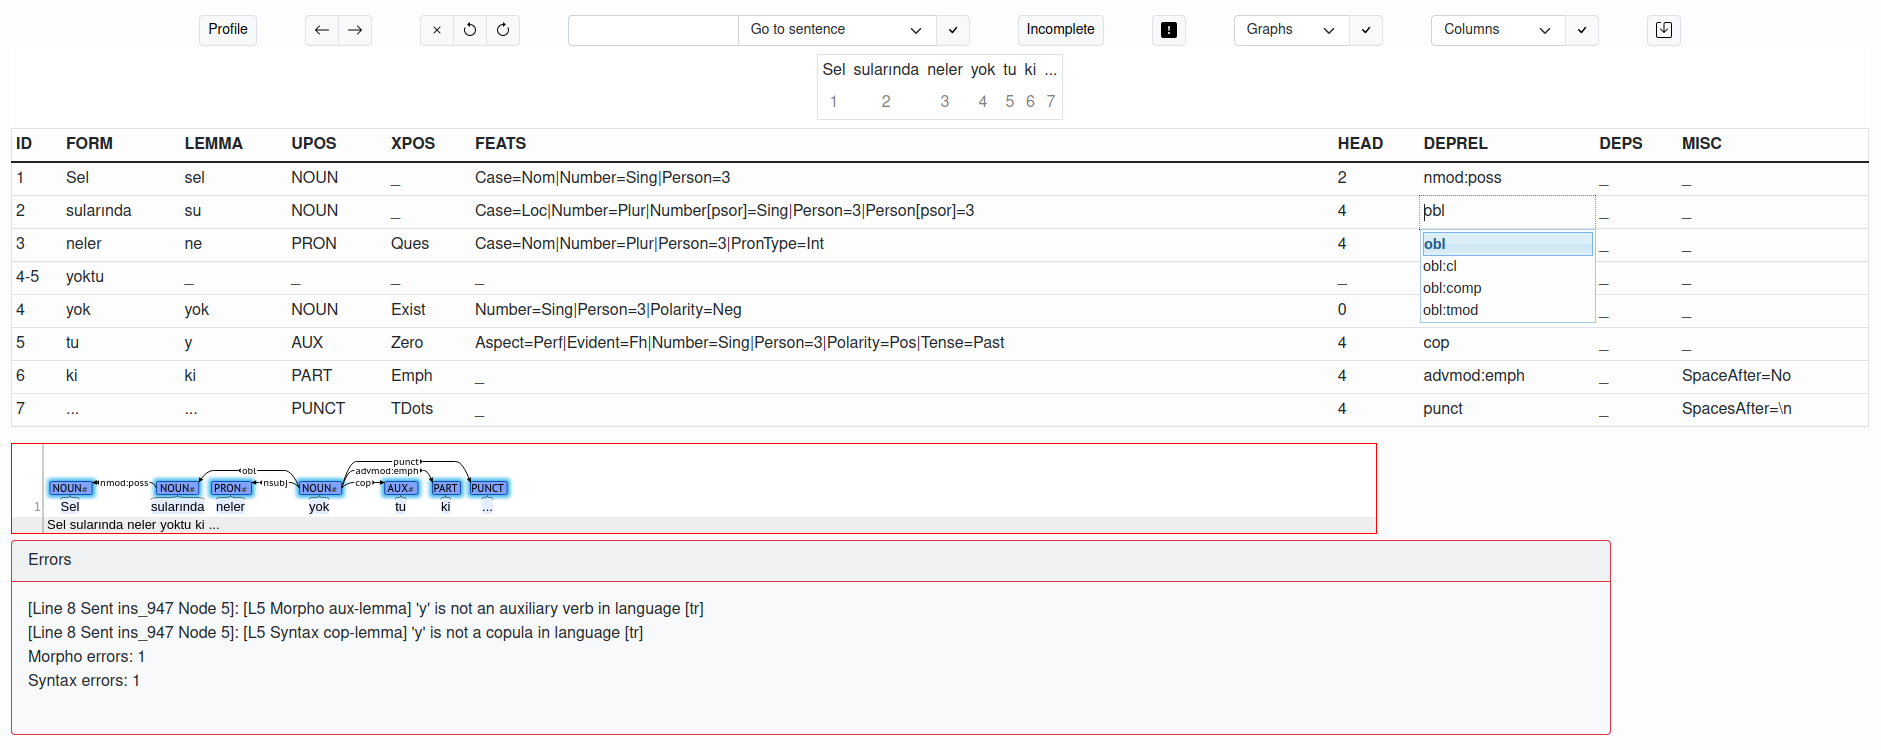
\includegraphics[width=0.6\textwidth]{1.png}
\caption{Once upon a time, kids could not wait to get their hands on these booklets obtained from Dandy chewing gum.}
\label{fig:demo-fig}
\end{figure}

\section{Discussion}
\label{sec:discussion}

What could be done further?
% django selection
% interviews had influence on the work; important
% different, educational tool
% customization, dark mode

\section{Conclusion}
\label{sec:conclusion}
% with boat feedback, web version planned
% dockerized, implemented
% we believe it's helpful
% nlp website accessible

\begin{acknowledgments}
% check code
This work was supported by Boğaziçi University Research Fund Grant Number 16909.
\end{acknowledgments}

\bibliography{main}

\end{document}
